% Extensión estimada: 3--3.5 páginas, cinco subsecciones y una tabla de correspondencia.
% Fuentes: scripts/robustness_perturbations.py; scripts/posthoc_calibration.py; scripts/interpretability.py;
% scripts/measure_cost.py; outputs/results/{lesion_split_report, robustness/robustness_summary, cost/cost_comparison,
% *_hiba_test_results}.json; docs/resul/revision_experimentacion_20261003.md.
% Revisión del autor del 18/10/2026: reemplaza a la antigua Sección 3.9 (Análisis complementarios). Las pruebas
% estadísticas pasaron a 3.7 (sec:met_estadistica).
% Revisión del tutor del 21/10/2026: una subsección por tipo de evaluación (generalización, robustez, calibración,
% interpretabilidad, costo), cada una con objetivo, procedimiento y métrica; el hardware de la medición de costo pasa
% a 3.9; cierra con la tabla que relaciona cada experimento con su objetivo y su métrica.

\section{Evaluaciones complementarias}
\label{sec:met_complementarios}

El conjunto de prueba de \emph{HAM10000} mide el desempeño en condiciones parecidas a las del entrenamiento: las imágenes
tienen el mismo origen y se capturaron y etiquetaron de la misma forma. Sin embargo, el tercer objetivo específico pide
evaluar los modelos en escenarios en que esas condiciones cambian (Sección~\ref{sec:marco_generalizacion}), y conocer
cuánto se puede confiar en sus salidas y cuánto cuesta ejecutarlos. Las evaluaciones de esta sección responden esas
preguntas y forman tres grupos. Las tres primeras estudian cómo cambia el desempeño de los clasificadores, según la
partición de los datos, en otro conjunto de datos y con imágenes degradadas. Las dos siguientes analizan otras
propiedades del clasificador: la confianza de sus probabilidades y la región de la imagen en que se apoya. La última
estima el costo de ejecutar los modelos y el \emph{pipeline}. Salvo que se indique otra cosa, se usan los modelos
elegidos en la Sección~\ref{sec:met_supervisados}, en su ejecución de referencia
(Sección~\ref{sec:met_estadistica}).

\subsection{Efecto de la fuga de información}
\label{sec:met_fuga}

La primera evaluación estima cuánto sobreestimaba el desempeño de los clasificadores la fuga de información que la
partición por lesión elimina (Sección~\ref{sec:met_particiones}). Para estimarlo, se compara el resultado de un
Swin-Tiny entrenado con la partición original sobre su conjunto de prueba completo con el que obtiene sobre las 894
imágenes cuya lesión no aparecía ni en entrenamiento ni en validación. Como control se usa DermLIP sin ajuste, que no
se entrenó con \emph{HAM10000}: si su desempeño también cambia entre ambos grupos, el cambio se atribuye a la composición
del subconjunto y no a la fuga.

\subsection{Generalización a otro conjunto de datos}
\label{sec:met_hiba}

La segunda evaluación busca saber si el desempeño se sostiene en un conjunto de datos distinto del de entrenamiento. Para
ello, Swin-Tiny y ConvNeXt-Tiny se evalúan sin ningún ajuste sobre las 1\,616 imágenes de \emph{HIBA}
(Sección~\ref{sec:met_datasets}), y la sensibilidad macro de cada uno se compara con la que obtiene en el conjunto de prueba de
\emph{HAM10000}. Como \emph{HIBA} mezcla imágenes dermatoscópicas y clínicas, el resultado también se separa por
modalidad. Parte de la diferencia, sin embargo, puede deberse al mapeo de diagnósticos, que lleva el carcinoma
escamoso a AKIEC, y no al cambio de conjunto de datos. Esa fuente de ruido no puede separarse, y por ello se declara.

\subsection{Robustez a perturbaciones de la imagen}
\label{sec:met_robustez}

La tercera evaluación mide qué ocurre si empeoran las condiciones de captura sin cambiar de conjunto. Con este
propósito, y siguiendo el esquema de los bancos de prueba de corrupciones de imagen~\cite{hendrycks2019benchmarking},
a las 1\,503 imágenes de prueba se les aplican cuatro perturbaciones, con cinco niveles de intensidad cada una:
compresión JPEG (calidad de 70 a 5), ruido gaussiano (desvío de 8 a 64 sobre la escala de 0 a 255), desenfoque
gaussiano (radio de 1 a 6 píxeles) y reducción de la resolución (de 0.75 a 0.15 del tamaño de entrada, de $224 \times 224$ píxeles, y vuelta a ese tamaño). La métrica es la caída relativa de la sensibilidad macro frente a la imagen sin perturbar
(Ecuación~\ref{eq:marco_robustez}). La Figura~\ref{fig:met_perturbaciones} muestra cómo queda una misma imagen con cada perturbación en los niveles 1, 3 y
5, es decir, qué degradaciones se evalúan. A diferencia de la evaluación principal, esta evaluación usa una sola vista de la
imagen, sin \gls{tta}.

\begin{figure}[H]
    \centering
    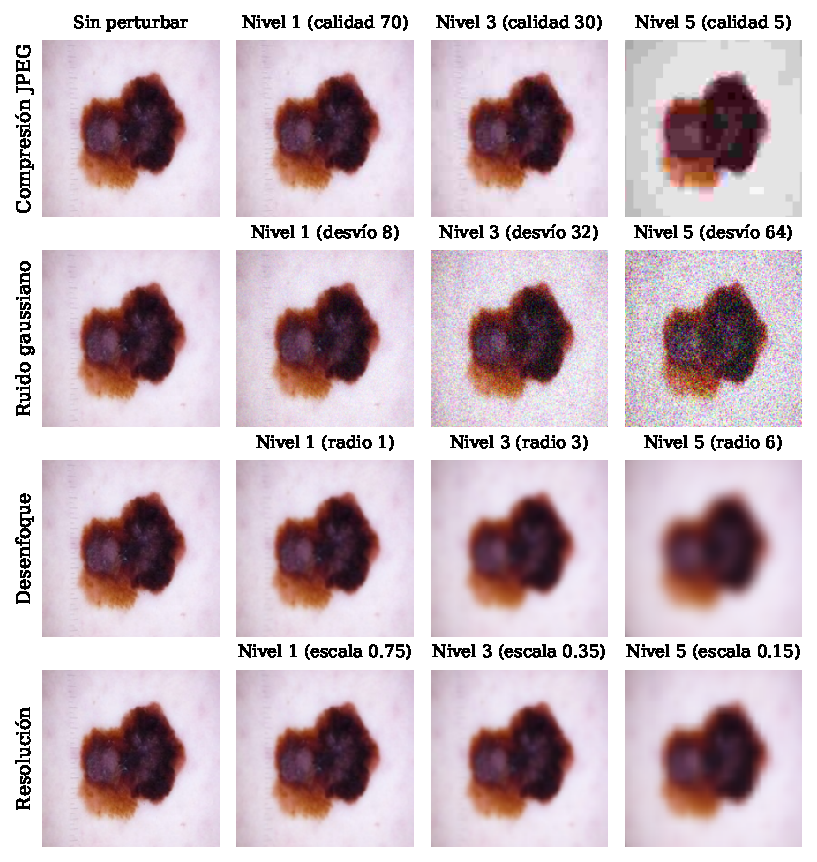
\includegraphics[width=0.72\textwidth]{Figures/Capitulos/03-Materiales-Metodos/perturbaciones-ejemplo.pdf}
    \caption{Una imagen del conjunto de prueba con cada perturbación de la evaluación de robustez, en los niveles 1, 3 y 5.}
    \label{fig:met_perturbaciones}
\end{figure}

\subsection{Calibración}
\label{sec:met_calibracion}

La cuarta evaluación busca saber cuánto se puede confiar en la probabilidad que da el modelo, que fija el umbral de
melanoma y que un clínico leería como certeza. Para ello se miden el ECE y el Brier
(Sección~\ref{sec:marco_eval_calib}) sin calibrar y con dos ajustes posteriores, \emph{temperature scaling} y
\emph{vector scaling}, que se ajustan en validación y se evalúan en el conjunto de prueba. Como el modelo guarda las
probabilidades promediadas con \gls{tta} y no sus salidas previas a la softmax, ambos ajustes se aplican sobre el
logaritmo de esas probabilidades, una aproximación que se declara. Además, dado que los pesos por clase alteran la
confianza del modelo, se comparan dos versiones de la misma configuración, entrenadas con y sin ellos.

\subsection{Interpretabilidad}
\label{sec:met_interpretabilidad}

La quinta evaluación examina en qué parte de la imagen se apoya el modelo. Para ello se aplica Grad-CAM
(Sección~\ref{sec:marco_eval_gradcam}) a Swin-Tiny, sobre la última etapa de la red y para la clase predicha, en siete imágenes de prueba, una por clase, con una sola vista, y en dos errores seleccionados entre los de activación
más alejada del centro de la imagen. Es una inspección cualitativa, que muestra si la activación cae sobre la lesión,
pero no mide el acierto ni respalda un razonamiento clínico.

\subsection{Costo computacional}
\label{sec:met_costo}

La última evaluación estima el costo computacional de ejecutar los modelos y el \emph{pipeline}, que es parte de la
restricción de la Sección~\ref{sec:met_tareas}. Para los clasificadores se miden los parámetros, la memoria máxima en
la GPU, el tiempo por imagen y las imágenes procesadas por segundo. Para los generadores, en cambio, se mide la memoria máxima al generar y se toma el tiempo por reporte de las ejecuciones
de la generación, que comparten instrucción, decodificación y límite de tokens,
de modo que la diferencia refleja el modelo y la longitud de lo que escribe. No es una medición controlada, sino una
estimación del orden de magnitud, que permite contrastar el \emph{pipeline} con el cómputo que usan los trabajos
revisados (Tabla~\ref{tab:marco_brechas} del Capítulo~\ref{cp:marco}). Las condiciones de la medición se detallan en
la Sección~\ref{sec:met_entorno}.

Con estas evaluaciones, quedan definidos todos los experimentos del trabajo, y falta ordenarlos según la parte del
problema que aborda cada uno.
